This chapter explores how altering the frequency with which the \cycamore reactor interacts with the \gls{dre} in \cyclus impacts the computational efficiency of a simulation and how to make the power output from a reactor more realistic.

\section{Archetypes and Time Management}
\label{sec:archetypes_and_time_management}

Throughout the \cyclus ecosystem, archetypes interact with the \gls{dre} and
each other in a fixed, user-defined time step, forcing the entire simulation
to operate on the smallest universal time step. For example, if a fabrication
facility can produce material every 2 months but the enrichment facility can
only provide material every 3 months, \cyclus would need to use a 1-month time step to capture both. When the time step is smaller than the minimum for a given
facility, that facility still participates in the \gls{dre} with a zero bid.
These zero bids, across hundreds of facilities, add complexity and
inefficiencies to solving the transaction problem at each time step.

In the \cyclus ecosystem there is an archetype called \textit{PatternSink} wherein the user can alter the frequency at which the sink, often called the repository, can accept the material. Figure \ref{fig:a-b-c} outlines an example scenario for this archetype with a simple A-B-C flow path. In this scenario, material is received from a source (A) to a reactor (B) with a final (C) sink that can only accept material at a specific frequency.

\begin{figure}[H]
    \centering
    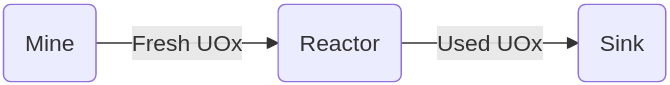
\includegraphics[scale=0.4]{images/cyclus/a-b-c.png}
    \caption{Simple A-B-C scenario.}
    \label{fig:a-b-c}
\end{figure}

Examining the material that the sink receives, it becomes clear that this
frequency alters how frequently the archetype updates its internal
understanding of time. It appears in Figure \ref{fig:pattern_freq_50} as though
multiple groups of material are received in one time step despite this
archetype not having an idea of individual shipments. This archetype
accomplishes the artificial restriction on accepting material by simply not
updating the time step that the archetype is at until the next universal time
step is met. Regardless of function, this is the only example of the
timekeeping flexibility found in the ecosystem.

\begin{figure}[H]
    \centering
    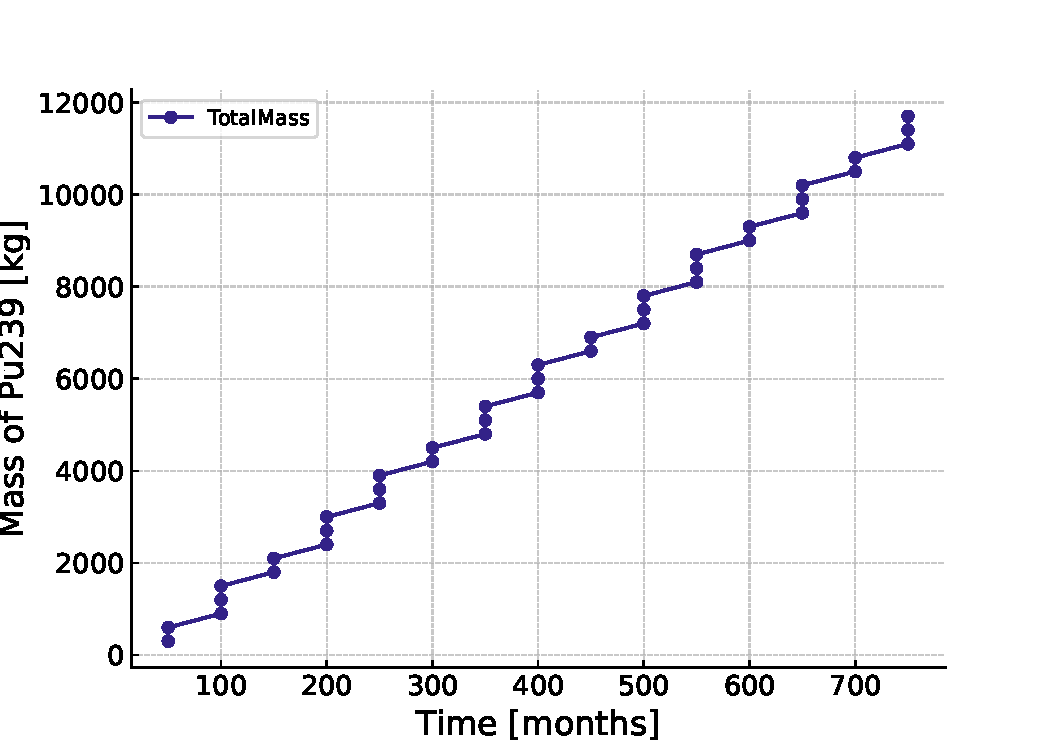
\includegraphics[scale=0.7]{images/cyclus/pattern_sink_fuel_transactions.pdf}
    \caption{Acceptance of $^{239}$Pu into the Sink with a frequency of 50 months.}
    \label{fig:pattern_freq_50}
\end{figure}

While archetypes like \textit{PatternSink} introduce new internal capabilities, they all inherit a set of base capabilities from the \cyclus toolkit. The \cyclus toolkit provides a modular and extensible framework for modeling \glspl{nfc}, allowing users to create custom archetypes that simulate various facilities and processes. These base capabilities standardize how archetypes create material buffers, interact with the \gls{dre}, and connect to the internal clock of the simulation, which are essential for coordinating the agents and commodities across their complex interactions within an \gls{nfc}. This thesis examines the fundamental capabilities of the \cyclus ecosystem and identifies time-intensive components of the current \cycamore Reactor. Section \ref{sec:trading_reactor} of this thesis creates an archetype called the \gls{tod} reactor, that interacts with the \gls{dre} only when it is time to refuel.

The toolkit’s modular architecture allows users to integrate new archetypes and models, promoting innovation and collaboration within the \cyclus community. This thesis contributes a reactor archetype called \gls{dpr} to the ecosystem that can adjust the power of the reactor based on user inputs to better capture real fluctuations in reactor operation. Through this archetype, this thesis explores incorporating historical realism and allowing for small timescale simulations to better capture the power output dynamics of the reactor fleet.

\section{Trading On-Demand Reactor}
\label{sec:trading_reactor}
% Review the literature related to the third subtopic. Summarize key findings and highlight important studies.

% Start with Cyclus time, go into pattern sink, and then archetype time toolkit update.
As Section \ref{sec:archetypes_and_time_management} discusses, \cyclus simulations have a universal time step at which every facility operates. The \cycamore reactor, like other archetypes, operates on this universal time step and interacts with the \gls{dre} at every time step. This interaction is necessary for the reactor to receive fuel and to bid on material from other facilities. However, this interaction is not necessary if the reactor does not need to refuel.

% Normal reactor
% 5,202,746,245 (52.57%)  => /home/rhysmac/cyclus/src/exchange_manager.h:cyclus::ExchangeManager<cyclus::Material>::Execute() (24x)
% 1,312,800,228 (13.26%)  => ???:cycamore::Reactor::Tock() (18,000x)
% 461,172,309 ( 4.66%)  => ???:cycamore::Reactor::Tick() (18,000x)
Valgrind's \cite{valgrind} Callgrind \cite{callgrind} tool profiles a source-reactor-sink scenario and establish which parts of the \cycamore reactor code generate the most instructions. 52.27\% of the 9,897,385,005 instructions come from the exchange manager in \cyclus, and the reactor's tock (which appends each time step) is the source of 13.26\% of the instructions. The reactor's tick (which pre-pends each time step) is the source of 4.66\% of the instructions.

The basic structure of each time step is fundamental to aligning the material transactions and bids in the existing \gls{dre}, so a reduction in computational cost could come from checking whether or not it is time to refuel before engaging with the calculations that take place when the reactor needs to refuel. This new archetype is called the \gls{tod} reactor, and the tock was the source of 11.5\% of the 9,519,845,814 instructions, while tick was the source of 2.77\% of the instructions.

% Silent reactor
% 5,083,560,026 (53.40%)  => /home/rhysmac/cyclus/src/exchange_manager.h:cyclus::ExchangeManager<cyclus::Material>::Execute() (24x)
% 1,094,637,634 (11.50%)  => ???:cycamore::SilentReactor::Tock() (18,102x)
% 264,086,388 ( 2.77%)  => ???:cycamore::SilentReactor::Tick() (18,102x)


There are ten duplicates in this thesis of a simple source-reactor-sink scenario to further compare how the \cycamore and \gls{tod} reactors perform and collected statistics with the Linux tool Perf \cite{perf}. In these scenarios, \cyclus deploys 1000 reactors over the first ten time steps, and the reactors operate for three time steps before refueling for two. This scenario demonstrates an intensive deployment to exacerbate the differences between the two reactor archetypes. The mean, maximum, minimum, and standard deviation of the wall clock time, number of instructions, and instructions per cycle are in Table \ref{tab:tod_profile}.

% make a table for the time_context max, min, average, and standard deviation
\begin{table}[H]
    \centering
    \caption{\gls{tod} reactor and \cycamore reactor profiles.}
    \label{tab:tod_profile}
    \begin{tabular}{l l l l l l}
        \hline
        Reactor & Metric & Mean & Max & Min & StDev\\
        \hline
        \cycamore Reactor & wall clock time [sec] & 3.286 & 3.333 & 3.242 & 0.026\\
         & Instructions & $1.209 \times10^{10}$ & $1.211 \times10^{10}$ & $1.207 \times10^{10}$ & $1.328 \times10^{7}$\\
         & Instructions per Cycle & 0.800 & 0.808 & 0.791 & 0.005\\
        \gls{tod} Reactor & wall clock time [sec] & 3.166 & 3.195 & 3.142 & 0.016 \\
        & Instructions & $1.174 \times10^{10}$ & $1.176 \times10^{10}$ & $1.167 \times10^{10}$ & $2.692 \times10^{7}$\\
         & Instructions per Cycle & 0.807 & 0.811 & 0.801 & 0.003\\
        \hline
    \end{tabular}
\end{table}

The results in Table \ref{tab:tod_profile} indicate an average speedup of 1.038, going from the \cycamore reactor to the \gls{tod} reactor. As Figure \ref{fig:time_violin} indicates, these time results are significant outside their combined standard deviations.

\begin{figure}[H]
    \centering
    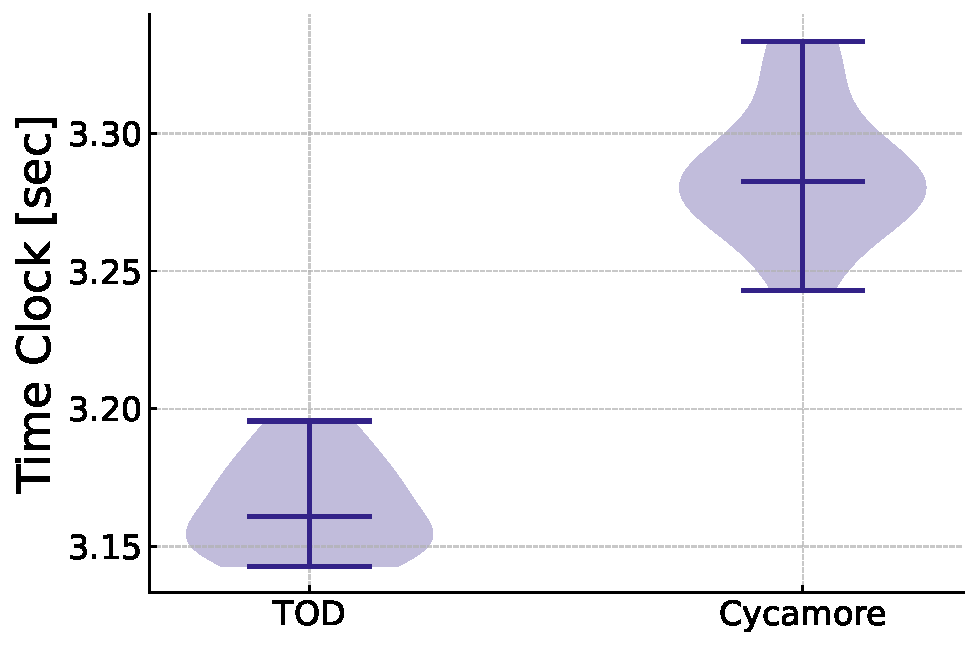
\includegraphics[width=0.7\linewidth]{images/power_reactor/time_clock_violin.pdf}
    \caption{Wall clock time values for the \gls{tod} and \cycamore reactors.}
    \label{fig:time_violin}
\end{figure}

The wall clock time values can vary by machine, architecture, and other demands during operation; however, the number of instructions issued using these archetypes, shown in Figure \ref{fig:isn_violin}, is distinct between the \gls{tod} and \cycamore reactors and is specific to the code, not the machine. The distributions of instructions per cycle, presented alongside the instructions, overlap but indicate that the average \gls{tod} reactor simulation has a higher utilization than the \cycamore reactor.

\begin{figure}[H]
    \subfloat[Number of instructions for \gls{tod} and the \cycamore Reactor.\label{fig:ins_tod_cyc}]{%
      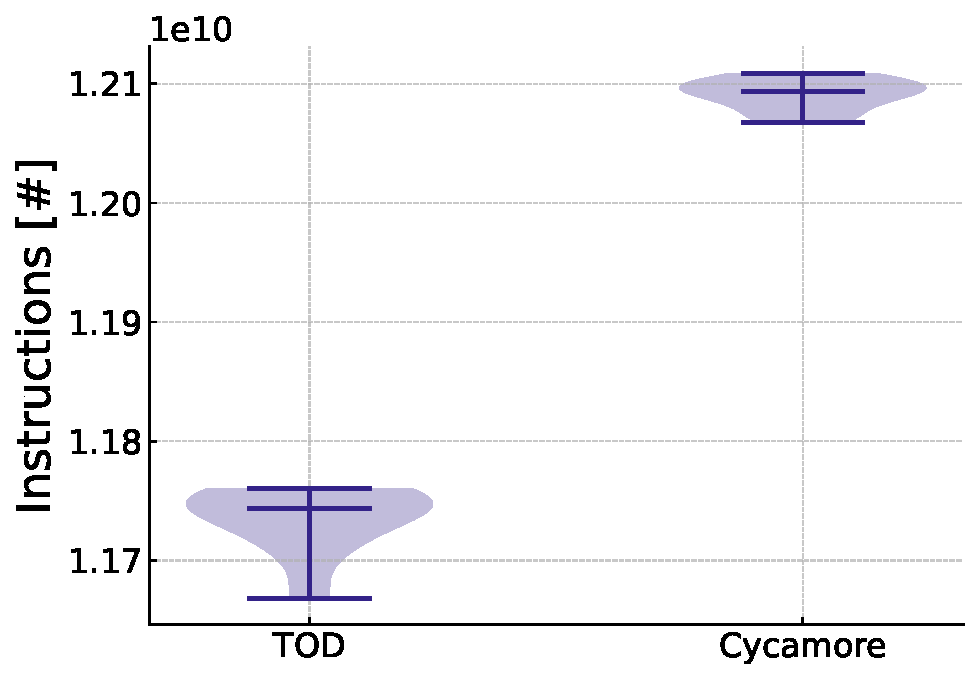
\includegraphics[width=0.49\textwidth]{images/power_reactor/ins_violin.pdf}
   }
    \hfill
    \subfloat[Number of instructions per cycle for \gls{tod} and the \cycamore Reactor.\label{fig:ins_per_cyc}]{%
      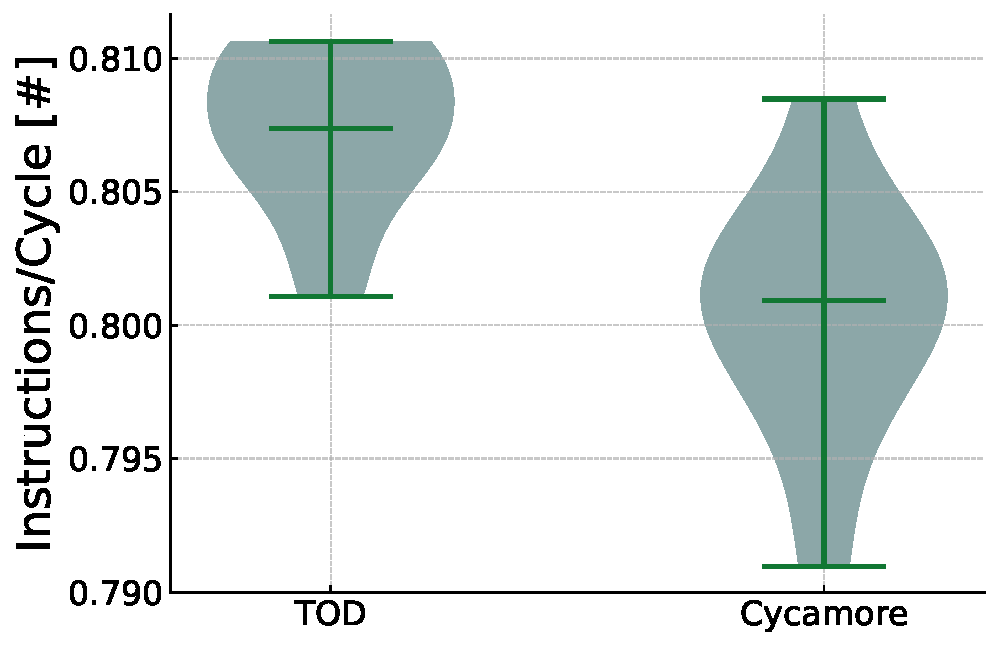
\includegraphics[width=0.49\textwidth]{images/power_reactor/ins_per_cyc.pdf}
   }
    \caption{Comparing the number of instructions and instructions per cycle for the \gls{tod} and \cycamore reactors shows that \gls{tod} has a higher utilization.}
    \label{fig:isn_violin}
\end{figure}